前章で設計したクラスを実装する.
%\vspace{5pt}
\subsection{MainActivity}

\begin{itemize}
 \item 親クラスをSetupに変更し,onCreate\footnote{Androidアプリケーションが立ち上がる際に実行されるメソッド}内で親クラスのsetupメソッドを実行している.
 \item それ以外の処理は無く,アプリケーションを立ち上げた際に一度だけ呼ばれるクラスとなっている.
\end{itemize}

%\vspace{5pt}
\subsection{Setup}
\begin{itemize}
 \item 親クラスはARActivity\footnote{ARToolKitの中枢クラス,ライブラリのクラスを制御している}で,アプリの起動,画面の作成,カメラからの画像の取得など初期設定を全て担っている.またRenderer\footnote{3Dオブジェクトを描写するクラス}をセットするなど描写方面の初期設定も同時に担っている.
 \item 基本的にこのクラスは初期設定を担っている為中身を変更する事はない.よってライブラリに付属させて配布する事が可能である.
\end{itemize}

%\vspace{5pt}
\subsection{AR}
\begin{itemize}
 \item 後述するDrawクラスで描画するBoxの情報をSetするメソッドである.DrawクラスのSetterをまとめたクラスと言える.コードの内容もほぼDrawクラスのSetterを呼び出して数値を設定しているだけである.
 \item わざわざSetterだけを分離した理由は,変更箇所を一まとめにする事で変更してはいけないところを間違って変更してしまうなどのミスが減らせる事などである.
\end{itemize}

%\vspace{5pt}
\subsection{Draw}

\begin{itemize}
 \item 前述したARクラスから値を受け取るGetterと後述するCubeクラスで設定したBoxを描写するクラスである.ARクラスから受け取った値を元にCubeクラスでBoxを作成し,マーカー上に描写する.
 \item このDrawクラスの描写をするメソッドを変更する事で様々な表現が可能である.しかし今回のコンセプトは``とりあえず拡張現実感を体験しよう''なのでここではBoxを表示するだけにとどめている.
\end{itemize}

%\vspace{5pt}
\subsection{Cube}
\begin{itemize}
 \item 受け取った数値を元に大きさ,色,透明度の情報を持つBoxを生成するクラスである.
 \item ここを変更する事で様々な形を表現する事が可能である.また3Dオブジェクトの表示も可能である.しかし前述した通りコンセプトに合わない為Boxの表示をする機能だけにとどめた.
\end{itemize}

\subsection{実行結果}
実行結果をFig.\ref{fig:res1}~-~Fig.\ref{fig:res3}に示す.Fig.\ref{fig:res1}は実行前,Fig.\ref{fig:res2}は色指定が(R, G, B, α)の時\footnote{いずれも最大値は255である}(0, 255, 0, 0),Fig.\ref{fig:res3}は色指定が(0, 255, 255, 100)の時である.また使用者が実際に改変するクラスであるAR.javaを以下に示す.

\begin{lstlisting}
package com.example.yuut.test6;
import org.artoolkit.ar.base.Draw;

public class AR extends Draw{

	public Draw MarkerID = new Draw();

	@Override
	public void setdraw(){
		MarkerID.setID("single;Data/patt.hiro;80");
		MarkerID.setColor(0, 255, 255, 100);
		MarkerID.setSize(1);
	}
}
\end{lstlisting}

\begin{figure}[tb]
\centering
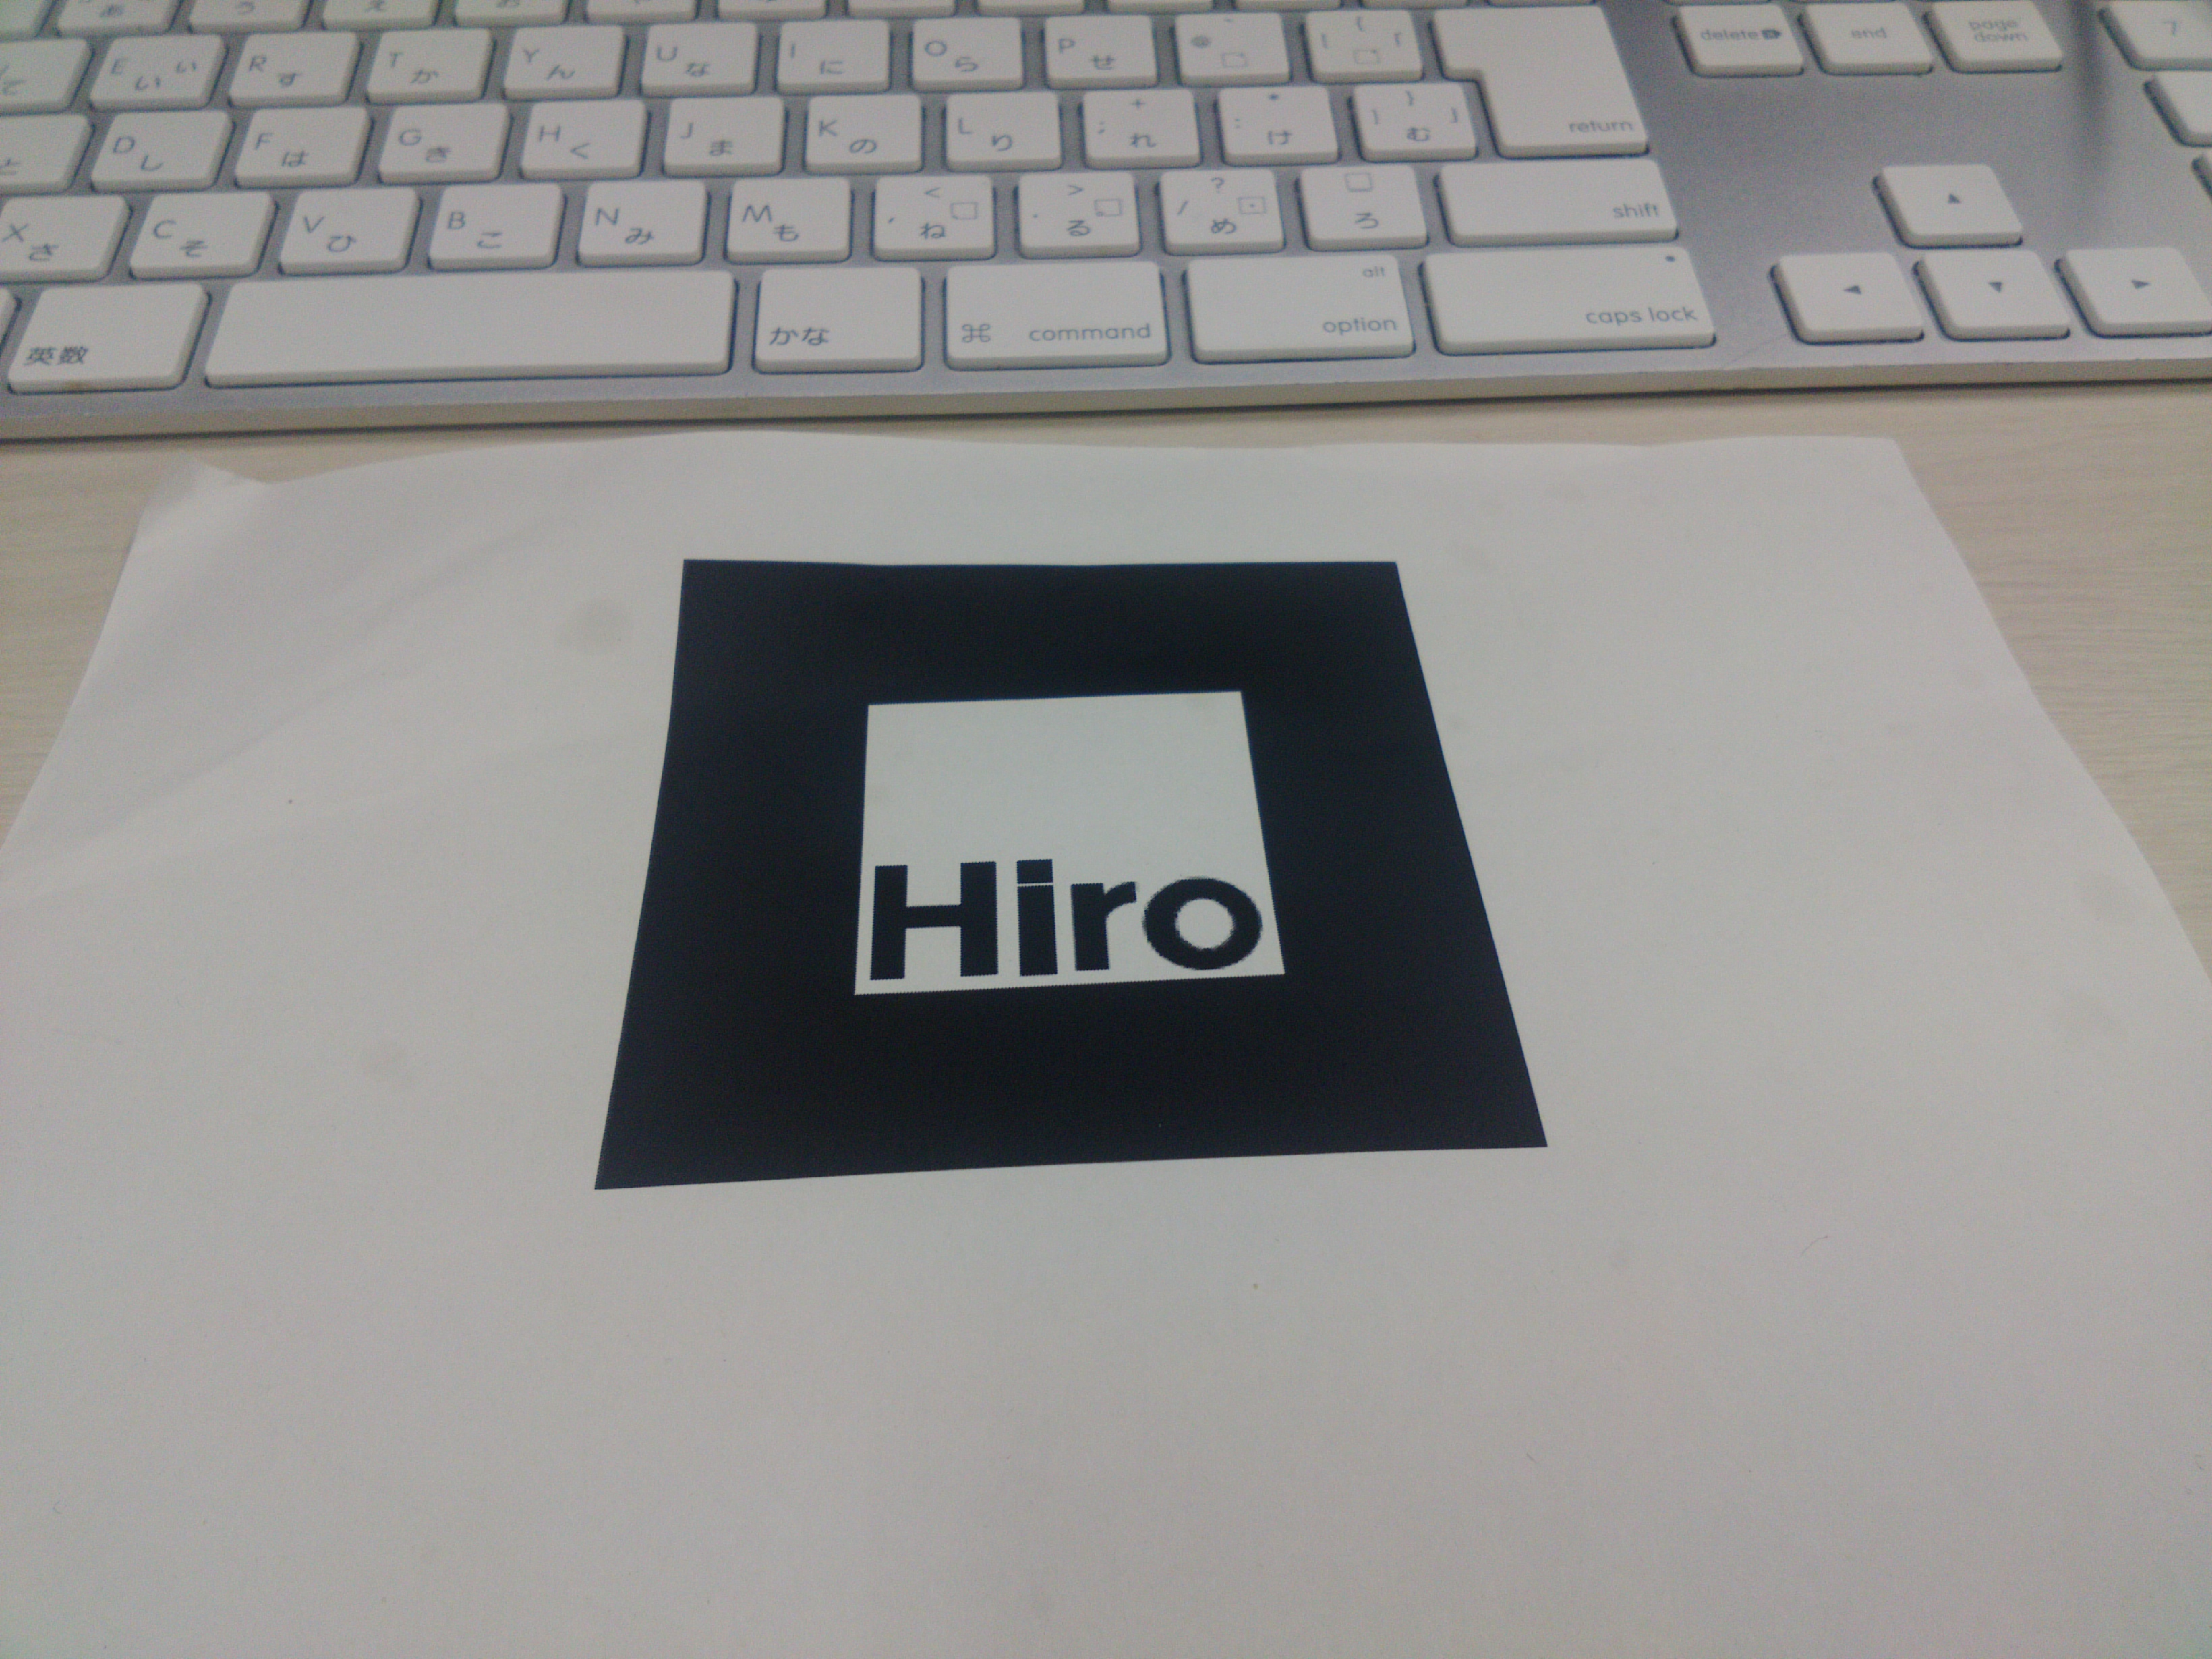
\includegraphics[width=9cm]{fig/res1.pdf}
\caption{Before execution}
\label{fig:res1}
\end{figure}
\begin{figure}[tb]
\centering
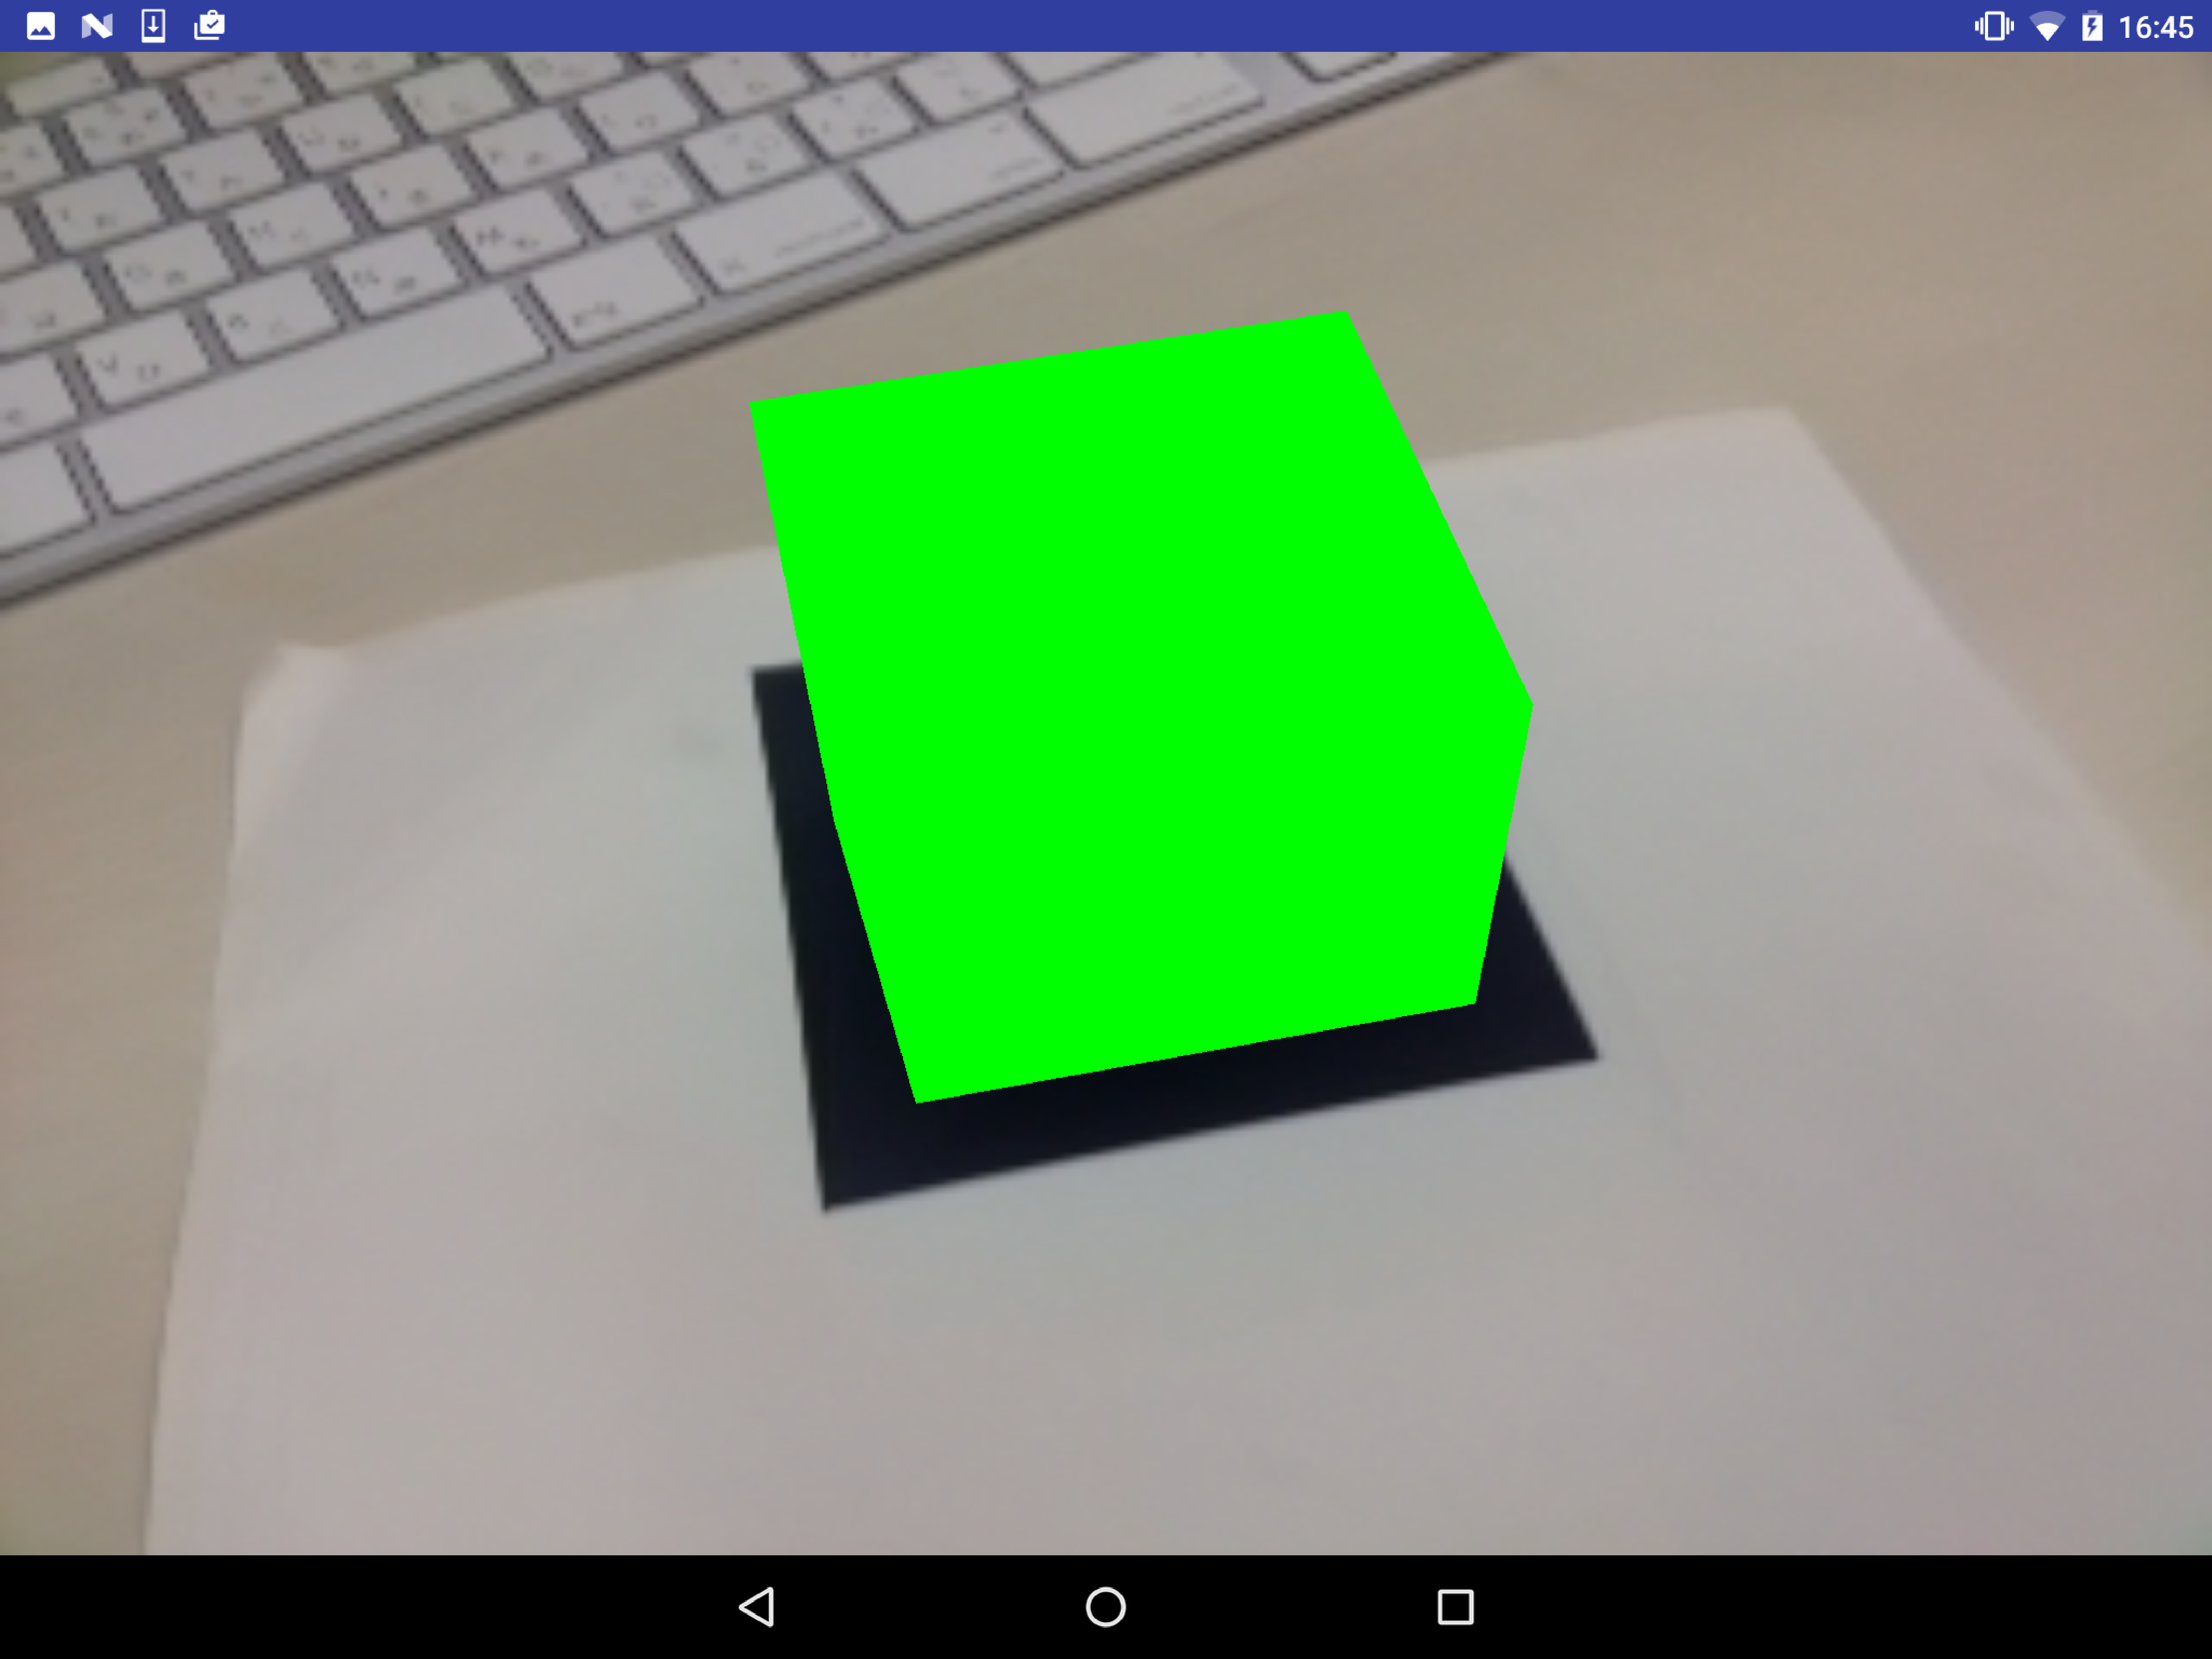
\includegraphics[width=9cm]{fig/res2.pdf}
\caption{Execution 1}
\label{fig:res2}
\end{figure}
\begin{figure}[tb]
\centering
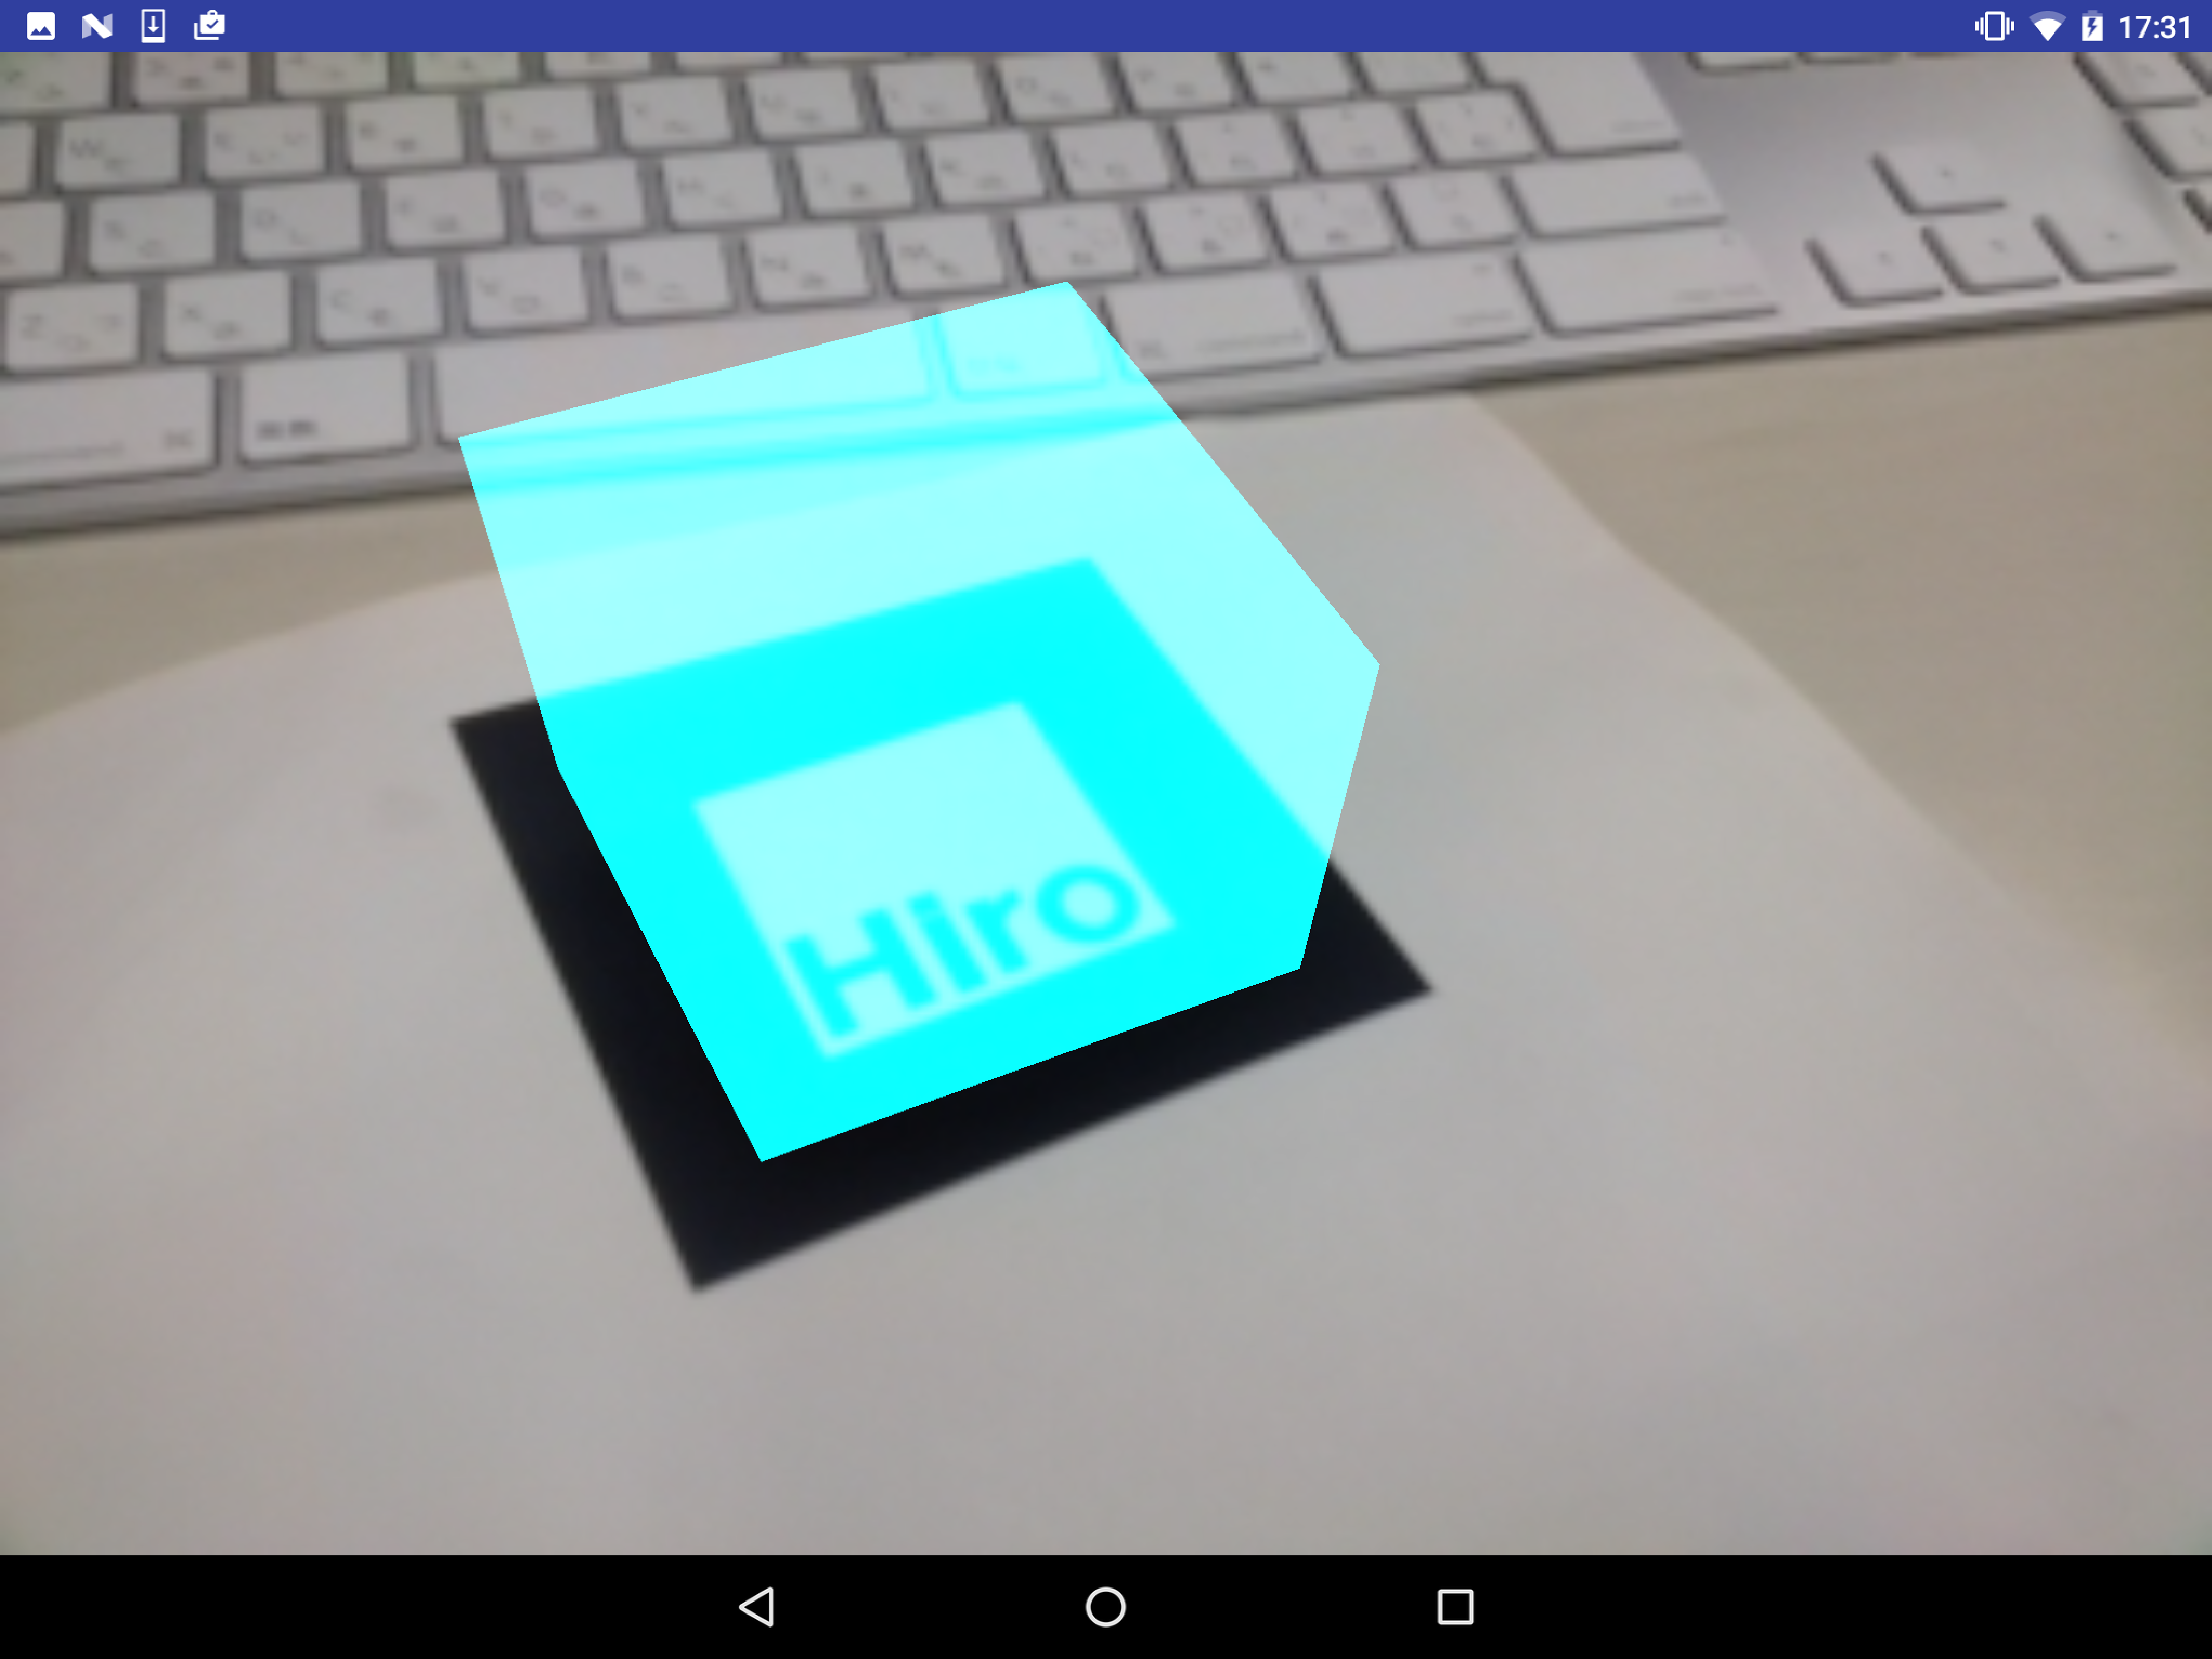
\includegraphics[width=9cm]{fig/res3.pdf}
\caption{Execution 2}
\label{fig:res3}
\end{figure}
\ 
\newpage